\documentclass[conference]{IEEEtran}

\usepackage{cite}
\usepackage{amsmath,amssymb,amsfonts}
\usepackage{graphicx}
\usepackage{textcomp}
\usepackage{xcolor}
\usepackage{listings}
\usepackage{float}
\usepackage{array}
\usepackage[hidelinks]{hyperref}

\definecolor{codegreen}{rgb}{0,0.6,0}
\definecolor{codegray}{rgb}{0.5,0.5,0.5}
\definecolor{codepurple}{rgb}{0.58,0,0.82}
\definecolor{backcolour}{rgb}{0.95,0.95,0.92}

\lstdefinestyle{mystyle}{
    backgroundcolor=\color{backcolour},
    commentstyle=\color{codegreen},
    keywordstyle=\color{blue},
    numberstyle=\tiny\color{codegray},
    stringstyle=\color{codepurple},
    basicstyle=\ttfamily\scriptsize,
    breaklines=true,
    captionpos=b,
    keepspaces=true,
    numbers=left,
    numbersep=5pt,
    showspaces=false,
    showstringspaces=false,
    showtabs=false
}

\lstset{style=mystyle}

\begin{document}

\title{Implementation of Single-Cycle RISC-V Processor in Verilog}

\author{
\IEEEauthorblockN{Hassan Raza (2024229), Emaan Swati (2024156)}
\IEEEauthorblockA{
 \\
Computer Organization and Assembly Language Lab \\
Date: 8 May 2026
}
}

\maketitle

%--------------------------------------------------

\begin{abstract}
RISC-V is a modern open-source Instruction Set Architecture (ISA) designed to provide simplicity, flexibility, modularity, and scalability in processor design. In this project, a Single-Cycle RISC-V Processor was implemented using Verilog HDL. The processor executes one instruction completely within a single clock cycle. The implemented processor supports arithmetic, logical, memory-access, and branch instructions including ADD, SUB, AND, OR, ADDI, LW, SW, and BEQ. Major hardware components including Program Counter, Instruction Memory, Register File, Control Unit, ALU Control Unit, Arithmetic Logic Unit, Data Memory, Immediate Generator, Multiplexers, and Adders were integrated into a complete datapath. Simulation and testing were performed using a Verilog testbench to verify correct processor functionality.
\end{abstract}

\begin{IEEEkeywords}
RISC-V, Verilog HDL, Single-Cycle Processor, ALU, Datapath, Computer Architecture
\end{IEEEkeywords}

%--------------------------------------------------

\section{Introduction}

RISC-V is an open-source Instruction Set Architecture (ISA) developed at the University of California, Berkeley. It provides a simple, modular, and extensible processor architecture for modern hardware design.

RISC-V follows the Reduced Instruction Set Computer (RISC) philosophy where instructions are simple and optimized for efficient hardware implementation. Because of its open-source nature, RISC-V is increasingly used in research, embedded systems, IoT devices, and processor development.

In this project, a Single-Cycle RISC-V Processor was implemented using Verilog HDL. In a single-cycle architecture, each instruction completes execution within one clock cycle. Although this design is not optimized for maximum performance, it provides a clear understanding of datapath organization and processor operation.

The processor supports arithmetic, logical, memory, and branch instructions and integrates all major datapath components into a complete processor architecture.

%--------------------------------------------------

\section{Objectives}

The objectives of this project are:

\begin{itemize}
    \item To understand RISC-V architecture and instruction formats.
    \item To understand instruction fetch, decode, execute, memory, and write-back stages.
    \item To implement processor modules using Verilog HDL.
    \item To design a complete single-cycle processor datapath.
    \item To simulate and verify processor functionality using a testbench.
\end{itemize}

%--------------------------------------------------

\section{Background Theory}

\subsection{RISC-V Architecture}

RISC-V is based on the Reduced Instruction Set Computer architecture. The ISA uses simple and fixed instruction formats that simplify hardware implementation.

Key features of RISC-V include:

\begin{itemize}
    \item Simple and modular architecture
    \item Open-source design
    \item Extensible instruction set
    \item Efficient hardware implementation
    \item High portability
\end{itemize}

\subsection{Single-Cycle Processor}

In a single-cycle processor, every instruction executes completely within one clock cycle.

Major stages include:

\begin{enumerate}
    \item Instruction Fetch
    \item Instruction Decode
    \item Execute
    \item Memory Access
    \item Write Back
\end{enumerate}

Advantages include simple control logic and easy debugging, while disadvantages include longer clock cycles.

%--------------------------------------------------

\section{Instruction Formats}

\subsection{R-Type Instructions}

R-type instructions are used for arithmetic and logical operations.

Supported instructions:

\begin{itemize}
    \item ADD
    \item SUB
    \item AND
    \item OR
\end{itemize}

\subsection{I-Type Instructions}

I-type instructions use immediate operands.

Supported instructions:

\begin{itemize}
    \item ADDI
    \item LW
\end{itemize}

\subsection{S-Type Instructions}

S-type instructions are used for memory store operations.

Supported instruction:

\begin{itemize}
    \item SW
\end{itemize}

\subsection{SB-Type Instructions}

SB-type instructions are used for branch operations.

Supported instruction:

\begin{itemize}
    \item BEQ
\end{itemize}

%--------------------------------------------------

\section{Implemented Instructions}

\begin{table}[H]
\caption{Implemented Instructions}
\centering
\begin{tabular}{|c|c|c|}
\hline
Instruction & Type & Description \\
\hline
ADD & R-type & Addition \\
SUB & R-type & Subtraction \\
AND & R-type & Logical AND \\
OR & R-type & Logical OR \\
ADDI & I-type & Add Immediate \\
LW & I-type & Load Word \\
SW & S-type & Store Word \\
BEQ & SB-type & Branch if Equal \\
\hline
\end{tabular}
\end{table}

%--------------------------------------------------

\section{Processor Architecture}

The processor follows the standard single-cycle datapath architecture.

\begin{figure}[H]
\centering
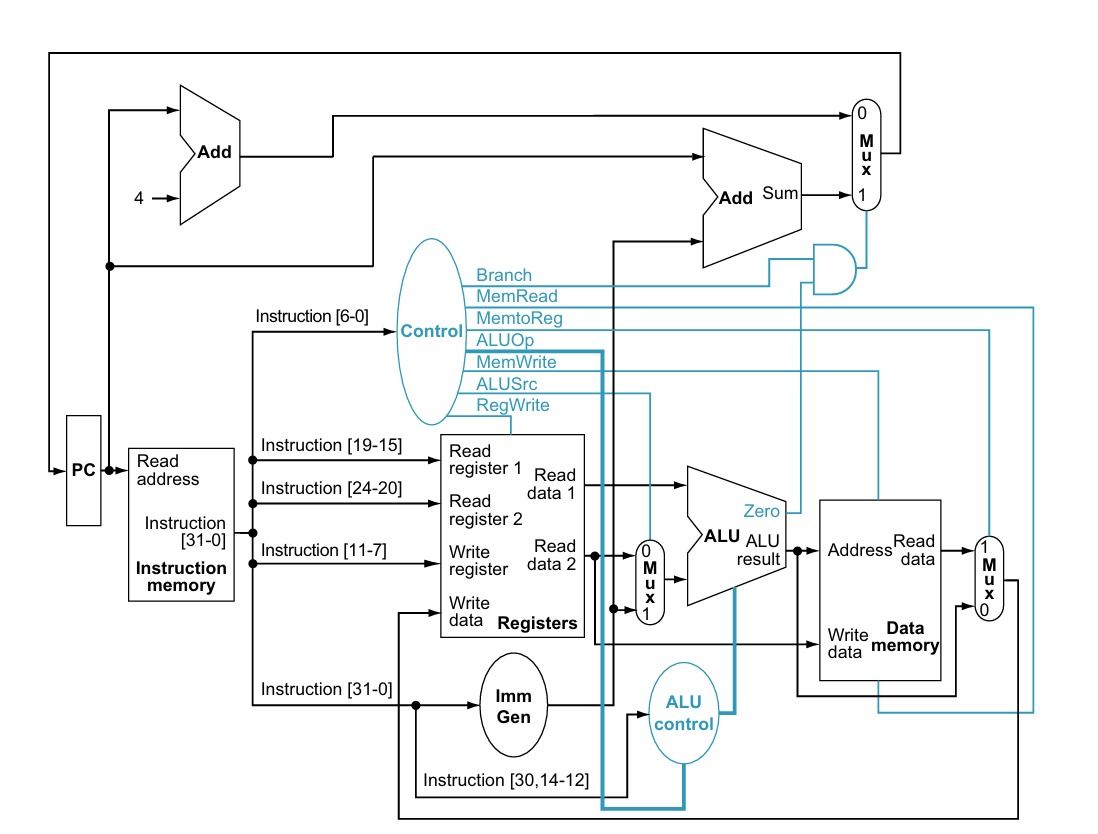
\includegraphics[width=0.98\linewidth]{WhatsApp Image 2026-05-07 at 20.28.35.jpeg}
\caption{Single-cycle processor datapath}
\label{fig:single-cycle-datapath}
\end{figure}

The datapath integrates:
\begin{itemize}
    \item Program Counter
    \item Instruction Memory
    \item Decoder
    \item Register File
    \item ALU
    \item Data Memory
    \item Multiplexers
    \item Adders
    \item Control Unit
    \item ALU Control Unit
\end{itemize}

%--------------------------------------------------

\section{Modules Description}

\subsection{Program Counter}

The Program Counter stores the address of the next instruction.

Functions include:
\begin{itemize}
    \item Holding current instruction address
    \item Updating instruction sequence
    \item Supporting branch operations
\end{itemize}



%--------------------------------------------------

\subsection{Instruction Memory}

Instruction memory stores machine instructions executed by the processor.

Sample instructions include:

\begin{itemize}
    \item addi x1, x0, 5
    \item addi x2, x0, 10
    \item add x3, x1, x2
    \item sub x4, x3, x1
    \item and x5, x3, x2
    \item or x6, x4, x2
    \item sw x3, 0(x0)
    \item lw x7, 0(x0)
    \item beq x7, x3, 4
\end{itemize}

%--------------------------------------------------

\subsection{Decoder}

The decoder extracts instruction fields from the 32-bit instruction.

\begin{table}[H]
\caption{Instruction Fields}
\centering
\begin{tabular}{|c|c|}
\hline
Field & Bit Range \\
\hline
Opcode & [6:0] \\
rd & [11:7] \\
funct3 & [14:12] \\
rs1 & [19:15] \\
rs2 & [24:20] \\
funct7 & [31:25] \\
\hline
\end{tabular}
\end{table}

%--------------------------------------------------

\subsection{Control Unit}

The control unit generates control signals according to the instruction opcode.

Generated signals include:

\begin{itemize}
    \item ALUSrc
    \item MemtoReg
    \item RegWrite
    \item MemRead
    \item MemWrite
    \item Branch
    \item ALUOp
\end{itemize}

\begin{table}[H]
\caption{Opcode Handling}
\centering
\begin{tabular}{|c|c|}
\hline
Opcode & Instruction Type \\
\hline
0110011 & R-Type \\
0000011 & LW \\
0100011 & SW \\
1100011 & BEQ \\
0010011 & ADDI \\
\hline
\end{tabular}
\end{table}

%--------------------------------------------------

\subsection{Immediate Generator}

The Immediate Generator extracts and sign-extends immediate values.

Supported formats include:

\begin{itemize}
    \item I-Type
    \item S-Type
    \item B-Type
\end{itemize}

For I-type instructions:

\[
Immediate = \{20\{instruction[31]\}, instruction[31:20]\}
\]

%--------------------------------------------------

\subsection{Register File}

The Register File stores operands and intermediate data.

Features include:

\begin{itemize}
    \item 32 general-purpose registers
    \item Two read ports
    \item One write port
    \item Register x0 always equals zero
\end{itemize}

%--------------------------------------------------

\subsection{ALU Control Unit}

The ALU Control Unit determines the required ALU operation.

\begin{table}[H]
\caption{ALU Operations}
\centering
\begin{tabular}{|c|c|}
\hline
ALU Control & Operation \\
\hline
0000 & AND \\
0001 & OR \\
0010 & ADD \\
0110 & SUB \\
\hline
\end{tabular}
\end{table}

%--------------------------------------------------

\subsection{Arithmetic Logic Unit}

The Arithmetic Logic Unit performs arithmetic and logical operations.

Supported operations include:

\begin{itemize}
    \item Addition
    \item Subtraction
    \item AND
    \item OR
\end{itemize}

Zero flag equation:

\[
Zero = (Result == 0)
\]

%--------------------------------------------------

\subsection{Data Memory}

The Data Memory performs load and store operations.

Features include:

\begin{itemize}
    \item 32 memory locations
    \item Synchronous write
    \item Asynchronous read
\end{itemize}

%--------------------------------------------------

\subsection{Multiplexers}

Multiplexers select data sources in the datapath.

Implemented multiplexers include:

\begin{itemize}
    \item ALU Source Multiplexer
    \item Memory-to-Register Multiplexer
\end{itemize}

%--------------------------------------------------

\section{Top Module Integration}

The \texttt{single\_cycle\_processor} module integrates all datapath components into a complete processor architecture.

Execution flow:

\begin{enumerate}
    \item PC provides instruction address
    \item Instruction memory fetches instruction
    \item Decoder extracts instruction fields
    \item Control unit generates signals
    \item Register file provides operands
    \item ALU performs operations
    \item Data memory handles memory instructions
    \item Results are written back to registers
\end{enumerate}

%--------------------------------------------------

\section{Branch Operation}

The processor supports the BEQ branch instruction.

Branch operation:

\begin{itemize}
    \item ALU subtracts two register values
    \item Zero flag determines equality
    \item Branch target address is calculated
    \item PC updates accordingly
\end{itemize}

\[
PC_{next} =
\begin{cases}
BranchTarget, & \text{if Branch AND Zero = 1} \\
PC + 4, & \text{otherwise}
\end{cases}
\]

%--------------------------------------------------

\section{Testbench}

A Verilog testbench was developed to verify processor functionality.

The testbench performs:

\begin{itemize}
    \item Clock generation
    \item Reset generation
    \item Output monitoring
    \item Waveform dumping
\end{itemize}

Monitored outputs include:

\begin{itemize}
    \item Program Counter
    \item Current Instruction
    \item ALU Result
    \item Register Outputs
    \item Data Memory Output
\end{itemize}

%--------------------------------------------------

\section{Simulation Results}

Simulation verified successful execution of all implemented instructions.

\begin{table}[H]
\caption{Simulation Results}
\centering
\begin{tabular}{|c|c|}
\hline
Instruction & Result \\
\hline
addi x1, x0, 5 & x1 = 5 \\
addi x2, x0, 10 & x2 = 10 \\
add x3, x1, x2 & x3 = 15 \\
sub x4, x3, x1 & x4 = 10 \\
and x5, x3, x2 & x5 = 10 \\
or x6, x4, x2 & x6 = 10 \\
lw x7, 0(x0) & x7 = 15 \\
\hline
\end{tabular}
\end{table}

%--------------------------------------------------

\section{Performance Analysis}

The implemented processor successfully executes all supported instructions in a single clock cycle. Since all stages of execution occur simultaneously within one cycle, the processor design remains simple and easy to debug.

The processor correctly handled:

\begin{itemize}
    \item Arithmetic computations using ADD and SUB instructions
    \item Logical operations using AND and OR instructions
    \item Immediate arithmetic using ADDI
    \item Memory access operations using LW and SW
    \item Branch decision making using BEQ
\end{itemize}

The branch mechanism was verified by comparing register values and updating the Program Counter accordingly.

Waveform analysis confirmed correct instruction sequencing and datapath operation.

%--------------------------------------------------

\section{Design Challenges and Debugging}

During implementation, several challenges were encountered while integrating processor modules into a complete datapath.

One major challenge was synchronization between the control unit and datapath modules. Incorrect control signals initially caused improper ALU operations and write-back behavior.

Another challenge involved immediate generation for branch instructions. Proper sign extension and branch target calculation were necessary for correct branching behavior.

Memory addressing also required debugging because the memory array was word-addressable.

Branch implementation required verification of:

\begin{itemize}
    \item ALU subtraction operation
    \item Zero flag generation
    \item Branch target calculation
    \item Program Counter update logic
\end{itemize}

Simulation waveforms and monitored outputs were used extensively during debugging.

%--------------------------------------------------

\section{Advantages}

Advantages of the implemented processor include:

\begin{itemize}
    \item Simple datapath organization
    \item Easy debugging and verification
    \item Straightforward control logic
    \item One-cycle instruction execution
    \item Useful for educational purposes
\end{itemize}

%--------------------------------------------------

\section{Limitations}

Limitations include:

\begin{itemize}
    \item Long clock cycle duration
    \item Lower performance compared to pipelined processors
    \item Inefficient hardware utilization
\end{itemize}

%--------------------------------------------------
%--------------------------------------------------

\section{Datapath Execution Flow}

The execution of an instruction inside the single-cycle processor follows a fixed datapath sequence. Every instruction passes through all stages of execution during one clock cycle.

\subsection{Instruction Fetch}

During the fetch stage, the Program Counter (PC) provides the address of the instruction to the instruction memory. The instruction memory outputs the corresponding 32-bit instruction.

The PC value is also incremented by 4 using an adder to point toward the next instruction.

\subsection{Instruction Decode}

In the decode stage, the decoder extracts the instruction fields including opcode, source registers, destination register, funct3, and funct7.

The control unit analyzes the opcode and generates control signals required for datapath operation.

At the same time, the register file reads operand values from the source registers.

\subsection{Execution Stage}

The ALU performs arithmetic or logical operations based on the ALU control signal.

For immediate instructions, the ALU receives the immediate value through the ALUSrc multiplexer.

For branch instructions, the ALU compares register values and generates the zero flag.

\subsection{Memory Access Stage}

For load and store instructions, the ALU output acts as the memory address.

\begin{itemize}
    \item LW reads data from memory
    \item SW writes data into memory
\end{itemize}

The memory module performs operations according to MemRead and MemWrite control signals.

\subsection{Write Back Stage}

The final stage writes data back into the register file.

The MemtoReg multiplexer selects whether the write-back value comes from:
\begin{itemize}
    \item ALU result
    \item Data memory output
\end{itemize}

This completes execution of the instruction within one clock cycle.

%--------------------------------------------------

\section{Control Signal Analysis}

Control signals are essential for coordinating datapath operations inside the processor.

The control unit generates signals depending on the instruction opcode.

\begin{table}[H]
\caption{Main Control Signals}
\centering
\begin{tabular}{|c|c|}
\hline
Signal & Function \\
\hline
ALUSrc & Selects ALU operand source \\
MemtoReg & Selects write-back source \\
RegWrite & Enables register writing \\
MemRead & Enables memory reading \\
MemWrite & Enables memory writing \\
Branch & Enables branch operation \\
ALUOp & Determines ALU operation type \\
\hline
\end{tabular}
\end{table}

For R-type instructions:
\begin{itemize}
    \item Register operands are selected
    \item ALU performs arithmetic/logical operations
    \item Result is written back to the register file
\end{itemize}

For load instructions:
\begin{itemize}
    \item Immediate value is added to base address
    \item Data memory performs read operation
    \item Loaded value is written back into a register
\end{itemize}

For store instructions:
\begin{itemize}
    \item ALU calculates memory address
    \item Register data is written into memory
\end{itemize}

For branch instructions:
\begin{itemize}
    \item ALU compares register values
    \item Zero flag determines branch decision
    \item Program Counter updates accordingly
\end{itemize}

\section{Conclusion}

A complete Single-Cycle RISC-V Processor was successfully implemented using Verilog HDL.

Major datapath components including Program Counter, Instruction Memory, Register File, ALU, Control Unit, Immediate Generator, and Data Memory were integrated into a complete processor architecture.

Simulation results verified successful execution of arithmetic, logical, memory, and branch instructions.

The project provided strong understanding of:

\begin{itemize}
    \item Processor datapath organization
    \item Instruction execution flow
    \item Control signal generation
    \item Hardware implementation using Verilog HDL
    \item RISC-V instruction formats
\end{itemize}

%--------------------------------------------------

\section{Future Improvements}

Future enhancements may include:

\begin{itemize}
    \item Pipelined processor architecture
    \item Hazard detection unit
    \item Forwarding unit
    \item Cache memory implementation
    \item Support for additional RISC-V instructions
    \item Performance optimization
\end{itemize}

%--------------------------------------------------

\begin{thebibliography}{00}

\bibitem{b1} RISC-V Foundation, ``The RISC-V Instruction Set Manual.''

\bibitem{b2} David Patterson and John Hennessy, \textit{Computer Organization and Design}, Morgan Kaufmann Publishers.

\bibitem{b3} Samir Palnitkar, \textit{Verilog HDL: A Guide to Digital Design and Synthesis}.

\bibitem{b4} Lab Manual: Implementation of RISC-V Processor in Verilog.

\end{thebibliography}

\end{document}